\input{chapter-header.tex}
% =============================================================================
\chapter{Introduction}
\chaplabel{introduction}
\minitoc
% =============================================================================


%Reflective systems are those that reason about and act upon themselves \cite{Smit84a}. A causal connection exists between the program and its representation inside the program itself as a meta-program \cite{Maes87a}. This reflective architecture introduces self-references:  an object-oriented system is composed by objects, which are instances of classes, which are also objects, and so on. These self-references, also known as meta-circularities \cite{Chib96a}, allow the manipulation of several meta-levels on one infrastructure.
%
%Reflective systems traditionally modify their self-representation to evolve and define new abstractions. However, the self-modification approach of evolution has many drawbacks, such as making difficult the self-surgery operations~\cite{Casa09a} or the lose of the reproducibility of the system. On the other hand, non-reflective systems develop an evolution approach by recreation. Whenever a change has to be made to the system, a new system is created with the new changes applied. This approach solves many of the drawbacks of the reflective approach.
%
%\gp{add some sentences on why it is important to evolve, which kind of software artifacts we would like to evolve, why it is challenging}

% =============================================================================
%\section{The need for Software Evolution}
% =============================================================================

An application runtime is the set of software elements that denote an application during its execution. Narrowing to high-level object-oriented applications, an application runtime includes \eg loaded libraries, classes and methods, created objects and threads. Within an application runtime, we find the \emph{language runtime}. The language runtime is the subset of the application runtime that defines the concepts and behavior available in the language we use \ie the set of structures and constructs that describe the language internals. The language runtime implements the model that the language proposes to the developers.

Manipulating and modifying these application and language runtimes, and therefore their language models, is becoming important in the last years. Multicore hardware brought new problems on concurrency and parallelism; the \emph{cloud} increases the need of software adaptation for application migration and resource tailoring; new resource constrained devices such as phones are widely spread, making ubiquitous computing a real concern. These new technologies present new challenges to software and language developers. The software we use, and in particular the programming languages and tools we use should be easily tailorable to support many of the new challenges that come with new technology and needs.

We observe, however, that software is not usually designed and thought to easily accept changes. Applications and languages should be either engineered from scratch with change in mind, or a lot of reengineering effort should be invested in them to perform changes. We need tools and methodologies that support such changes~\cite{Nier08b}. The languages and applications we develop should be adaptable to new situations and scenarios.

To address this goal we propose \emph{\Vtt}: a runtime virtualization infrastructure. \Vtt virtualizes an application runtime for its control and manipulation with the ultimate goal of generating specialized versions of it. Manipulations are transparent for the virtualized runtime. We show how \Vtt simplifies the generation of application and language runtimes in two different approaches: language runtime (re)creation by bootstrapping allows us to modify and redefine the concepts a language proposes to its users; application runtime extraction reduces the memory consumption caused by the code units of an application.

%For example, an application runtime should be easily tailorable to consume less resources. We can observe that deployed applications contain a set of \emph{code units} such as classes and methods that tend to occupy more memory~(primary and secondary) than necessary.
%This problem shows itself more evident and harder to control under the usage of third party software. 
%Third party libraries and frameworks are designed in a generic fashion that allows multiple usages and functionalities, while applications use only few of them. 
%Examples are logging libraries, web application frameworks or object-relational mappers.
%Unused code units represent serious drawbacks in constrained devices. 
%First, unused code units may forbid the deployment into a constrained resource device.
%It may also interfere with the deployment and usage of other applications, because of large memory footprints in both secondary~(disk storage) and primary~(RAM) memory~\cite{Mart12a} or the presence of slow networks in the case of rich web applications.
%Second, some deployment targets may have an infrastructure designed in such a manner that forbids the deployment of large applications. For example, the Android's Dalvik VM restricts an application to deploy only 65536 methods.


% =============================================================================
%\section{The cloud and Mobile code}
% =============================================================================

%\gp{explain why code mobility is important!}

%Another example of support that should be brought to user applications is \emph{code mobility}. Code mobility is a mechanism that allows the migration of programs between different environments. This problem is important in the context of ubiquitous systems and virtualization technology. Code mobility provides support for \eg load balancing, adjusting an application's resources dynamically and functionality customization. However, applications must have support to rebind a piece of code or object to another location~\cite{Fugg98a}.

\section{Motivation}

Advances in computing technology both in hardware and software demand that our applications and languages adapt themselves better to them. More resourceful machines can make use of richer programming languages with the purpose of enhancing the developer's productivity. We could think, for example, on extending an existing language with new concepts besides classes and inheritance such as first-class instance variables~\cite{Verw11a}. First-class instance variables provide a point of extension on instance variable access and allow the transparent implementation of alternative models for storing state~(\eg putting an object's state inside a dictionary instead of an object's slot). First-class instance variables help in removing boilerplate code and to provide better programming abstractions.

At the same time, constrained resource devices pose completely different challenges. Limitations in memory, energy or CPU power may require us to \emph{downgrade} some features from our applications and programs to reduce memory consumption. For example, we could think on removing the reflection support and the language meta-data from an application that does not use it. Moreover, we could think on removing every unused element from our application development artifact.

We believe applications and languages should provide support to tackle challenges as these ones. Moreover, they should not be limited to them but also be flexible to adapt themselves to other unknown situations.

% =============================================================================
\section{Application Runtimes: Concepts}
% =============================================================================

In the context of application runtime manipulation, we face the following question: \emph{What are the elements of high-level programming languages we should focus on?} High-level programs are inherent complex pieces of software. For such a reason in this thesis we narrow our study to those programs that run on top of a \VM because most of modern object-oriented languages~(\eg Java, Python, Ruby, JavaScript, C\#) are \VM-based.
This section proposes a dissection of a high-level language application runtime and states with it the terminology used during the rest of this dissertation. We made this dissection with the objective of understanding the relationship between the software elements. We believe that understanding these relationships is important in the context of this thesis. Figure \ref{fig:whatToEvolve} shows a schema of this dissection.

\begin{figure}[!ht]
\begin{center}
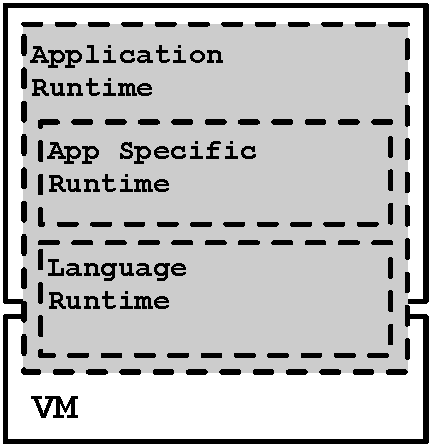
\includegraphics[width=0.5\linewidth]{elements_to_evolve}
\caption{\textbf{Dissection of a running program.}\label{fig:whatToEvolve} }
\end{center}
\end{figure}

An application runtime is the set of software elements that constitute an application during its execution. An application runtime includes software elements that describe the application's structure during its execution, such as its libraries, classes and methods, and elements related with the application's execution, such as threads, the execution stack with its activation records and created objects. We identify inside an application runtime two main components: the \emph{application specific} and the \emph{language} runtimes that represent respectively the elements of the application under execution and the language that provides support for it.

A Virtual Machine~(\VM) provides execution support for the application runtime. From the application runtime the distinction is usually clear: the language elements cannot arbitrarily access and modify the \VM elements. However, the opposite is not true. The \VM has complete power over the elements that belong to the application runtime. Moreover, this leads inside the \VM to a mixture between language and \VM concerns that blurs their relationship.
%In the context of this thesis, we do not consider the Virtual Machine as part of the application runtime, but as a machine that supports its execution.
Note that some authors may include the \VM inside a broader runtime system.
This is the reason why we use the terminology \emph{application runtime} instead of runtime system and we consider this component separately from the \VM.

\subsection{Language Runtime}

The subset of the application runtime that describes the language we use is the \emph{language runtime}. The language runtime includes the set of structures and constructs that describe the language concepts and behavior. This language runtime is the representation at runtime of the model that the language proposes to the developers. For example, Smalltalk and Ruby propose that an application is structured in classes with implicit metaclasses \ie a class is instance of a (\emph{meta-})class that describes its behavior. Therefore, they also contain structures that represent the concepts of a \ct{Class} and \ct{Metaclass} and control the implicit creation of a metaclass for each new class. Additionally, a language runtime is not only composed of classes but it also includes objects. For example, it contains a table of unique strings or \emph{symbols} used to univocally name objects. A language runtime is usually common to different applications in the same language: it is always present and contains always the same elements.

\subsection{Application Specific Runtime}

Within an application runtime we identify also the \emph{application specific runtime}. The application specific runtime is the subset of the application runtime that includes the elements that belong to the particular application. It contains, in other words, the classes written by the application developer. The application specific runtime follows the model and concepts imposed by the language \ie it is expressed in terms of the language runtime, and thus coupled to it. For example, the application specific classes of a Smalltalk or Ruby application have an implicitly created metaclass.

%\subsection{Virtual Machine}
%
%High-level languages virtual machines~(\VMs) provide support for executing an application runtime.
%Likewise, an application runtime must satisfy the \VM's interface to be executed.
%This interface denotes the \emph{execution model} of a \VM and includes the format in which the runtime elements are laid out in memory~(objects, classes, methods), the followed object model (\eg class-based or prototype-based) and the instruction set that the runtime must implement.
%
%\VMs concentrate several complex and interconnected elements with two main purposes: first it is to abstract applications from details such as memory management or machine specifics; second it is to do that while also obtaining good performance.
%Early \VMs focused on interpreting an abstract instruction set (bytecodes).
%On the one hand the bytecodes guarantee certain platform independence by abstracting away from the \CPU specific instruction set.
%On the other hand bytecodes allow one to encode complex operations into little space both serving the hard memory constraints of the hardware and simplifying the design of a compiler.
%Obviously this abstraction gain comes at a cost, and ever since the first \VMs were built, research and industry strive to reduce the interpretation overhead.
%
%%This goes even so far that specialized hardware is conceived to match the performance requirements \cite{Unga84a,Stef84a,McGh98a,Clic05a}.
%
%To improve performance some \VMs use a Just-In-Time compiler (\JIT) that dynamically generates native code from bytecode \cite{Deut84a}.
%In this case the bytecode becomes an intermediate representation (\IR) for a bigger compiler infrastructure.
%However, \JIT compilers are notoriously complex as they crosscut many \VM components and abstraction layers. They have to access high-level information from the running bytecodes and manage native code at the same time.
%Similar complexity applies to the automatic memory management present in most high-level language \VMs.
%Garbage Collectors (\GC) evolved from simple helpers to complex software artifacts that for instance support concurrent garbage collection \cite{Clic05a}.



%These complex \VMs are the enablers of many of the features in our programming languages.
%However, their complexity constrain the changes we can apply to our application runtimes.
%For example, adding a new field into the classes of an application runtime may impact the bytecode interpreter, the JIT, the GC, and so on.
%These constraints denote the \emph{execution model} of a \VM \ie the contract required to a language runtime to execute it.
%This execution model includes the format in which the runtime elements are layout in memory~(objects, classes, methods), the followed object model (\eg class-based or prototype-based) and the instruction set that the runtime must implement.

\section{Problem Statement}

This thesis focuses on the generation of specialized high-level object-oriented application and language runtimes for languages that run on a \VM. In this context, we aim at solving the following problems:

\begin{description}

\item[Extending languages.] The model proposed by a language is not always simple to change. Changing the concepts provided by a language may involve changes in its runtime or its \VM. Often, it requires us to have access to the \VM code, and forces us to modify such representation without the proper level of abstraction. Also, The relationship between the language and the \VM, particularly its execution model, often remains unclear. This unclear interface comes from hardcoded assumptions in the multiple \VM components. Its clients are exposed to the complexities of the \VM internals when it comes to change the application runtime.

\item[Reducing application runtime memory consumption.] The application specific part of an application runtime often embeds several libraries and elements from different origins \eg the language base libraries and third party libraries and frameworks. Reducing the memory consumption by removing unused elements such as classes and methods should ensure that the application works as expected at the end of such process. However, the absence of type annotations in dynamically-typed languages and the broad usage of dynamic features such as reflection makes this a challenging problem.


%\item[Mismatch between a language model and the \VM execution model.] The execution model imposed by a \VM is often more general than the particular languages that run of top of it. This means that a \VM can support different language models on top of it as long as they satisfy its execution model. However, the \VM often fixes the language model during its language initialization step, preventing us to easily modify it.

\end{description}

\noindent Then, we pose the following research question:

\begin{center}\emph{Is there a general purpose infrastructure that supports the creation of specialized application runtimes, particularly to extend a language model and/or reduce its memory consumption?}
\end{center}

We would like to have an infrastructure featuring safe application runtime manipulation, and allowing both the specialization and extension of application and language runtimes.

\section{Contributions}

To solve the stated problems, we make the following claim: \newline

\begin{center}\blockquote{\emph{Runtime virtualization and reification support the generation of specialized application and language runtimes, particularly to extend the language model and to discard unused runtime elements.}}
\end{center}

First-class runtimes should provide a clear and high-level \VM-Language interface. This interface must hide the internal details of the \VM complexities and allow us to easily manipulate the elements inside an application runtime. At the same time, it should ensure that the \VM execution model is honored during such manipulations.

The contribution of this thesis is three-fold. The main contribution is \Vtt, an \emph{infrastructure for application runtime virtualization}. This infrastructure allows us to manipulate and control a virtualized application runtime through a first-class runtime object, namely an object space.
We validate this language virtualization infrastructure by exploring two approaches for application runtime generation:
\begin{description}
\item[Language Runtime Bootstrapping.] We developed a bootstrapping process for an object-oriented high-level language. Bootstrapping is an explicit process that describes how a language runtime is created using the same language that it generates at the end. Bootstrapping provides us with full control on what are the elements installed in the application runtime at the end.
\item[Application Runtime Tailoring.] We developed a novel dynamic application runtime tailoring approach named Run-Fail-Grow~(RFG). RFG starts with an empty application runtime and it installs elements inside it as they are needed during at runtime. With RFG we can create a specialized runtime that contains only the used elements of an application.
\end{description}

% =============================================================================
\section{Thesis Outline}
% =============================================================================
%\sm{This dissertation structure is different to what I am used to. At least the way you announce the purpose of the chapters is not what I would expect.
%In my diss, everything revolves around one thesis, here, it is a number of things listed one after another, don't see the central motive I would expect}

\gp{write from scratch, left for the end}
\begin{description}
\item[\chapref{background}] 

\item[\chapref{benzo}] 
	
\item[\chapref{ffi}] 

\item[\chapref{validation}] 

\item[\chapref{conclusion}] 

\end{description}


% =============================================================================
\input{chapter-footer.tex}
% =============================================================================